\documentclass[11pt]{book}
\usepackage{fullpage}
\usepackage{longtable}
\usepackage{bytefield}
\usepackage{color}
\usepackage{graphicx}
\usepackage[table]{xcolor}
\usepackage[bookmarksopen=true]{hyperref}


\usepackage{sectsty}
\allsectionsfont{\usefont{OT1}{phv}{bc}{n}\selectfont}

\usepackage[Lenny]{fncychap}

\usepackage{fancyhdr}
\pagestyle{fancy}
\fancyhf{}

%% Now begin customising things. See the fancyhdr docs for more info.

\renewcommand{\chaptermark}[1]{\markboth{\MakeUppercase{#1}}{}}
\renewcommand{\sectionmark}[1]{\markright{\MakeUppercase{#1}}{}}
\renewcommand{\headrulewidth}{0pt}

\hypersetup{%
pdftitle={AjarDSP User's Guide},
pdfauthor={Markus Lavin <markusl.se78@gmail.com>},
pdfsubject={AjarDSP User's Guide},
pdfkeywords={AjarDSP}}

% Set up hyperlink colors
\definecolor{darkred}{rgb}{0.5,0,0}
\definecolor{darkgreen}{rgb}{0,0.3,0}
\definecolor{darkblue}{rgb}{0,0,0.5}
\definecolor{darkbrown}{rgb}{0.28,0.07,0.07}
\hypersetup{%
  colorlinks=true,
  citecolor=darkblue,
  urlcolor=darkgreen,
  linkcolor=darkred,
  menucolor=darkbrown}

\renewcommand{\familydefault}{\sfdefault}
\newcommand{\HRule}{\rule{\linewidth}{0.5mm}}

\begin{document}

\begin{titlepage}
\begin{center}
\HRule \\[0.4cm]
{\Huge \textbf{AjarDSP User's Guide}}\\[0.8cm]
\HRule \\[1.5cm]
\emph{URL:}\\
\texttt{http://code.google.com/p/ajardsp/}\\
\vfill
\begin{flushleft}
\begin{minipage}{0.4\textwidth}
\begin{flushleft} \large
\emph{Author:}\\
Markus Lavin \texttt{<markusl.se78@gmail.com>}
\end{flushleft}
\end{minipage}
\end{flushleft}
\end{center}
\end{titlepage}

\tableofcontents

\chapter{Architecture}
%\clearpage
\section{Overview}
AjarDSP is a 16-bit dual mac VLIW DSP. The major blocks of the DSP
core are depicted in figure \ref{ajardsp-blocks}.
\begin{figure}[!h]
  \scalebox{1}{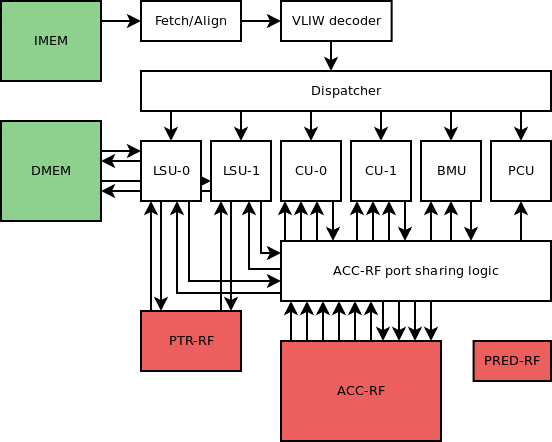
\includegraphics[scale=0.4, angle=-90, bb=20 20 842 700]{ajardsp-blocks.pdf}}
  \caption{\small AjarDSP blocks and interconnect.}
  \label{ajardsp-blocks}
\end{figure}
%\clearpage
\section{Registers}
This section describes the registers available in AjarDSP
architecture. There are two main register files (accrf and ptrrf) and
a group of loosely connected special purpose registers spread out
through the design called the special registers.
\subsection{Accumulator Register File (ACCRF)}
The accumulator register file (accrf) consists of eight 40-bit
accumulator registers. Each such accumulator register is divided into
three parts; guard bits (typically 8-bits but configurable), a 16-bit
high part and a 16-bit low part. See figure
\ref{accumulator-register}.  \break

\begin{figure}[!h]
\begin{bytefield}{40}
\bitheader[b]{0,15,16,31,32,39} \\
\bitbox{8}{accNg} &
\bitbox{16}{accNh} &
\bitbox{16}{accNl} \\
\end{bytefield}
\caption{\small 40-bit accumulator register.}
\label{accumulator-register}
\end{figure}

The high and low parts (accNh and accNl) may be addressed individually
by some instructions (those operating on 16-bit data) but the guard
bits are not directly addressable. Access to the guard bits must be
done via the BMU by means of downshifting.

The accumulator register file is equipped with a bypass network.

\subsection{Pointer Register File (PTRRF)}
The pointer register file (ptrrf) consists of eight 16-bit
registers. These registers are only accessible from the load store
units (LSU) and their purpose is to addressing memory. See figure
\ref{pointer-register}. \break

\begin{figure}[!h]
\begin{bytefield}{16}
\bitheader[b]{0,15} \\
\bitbox{16}{ptrN} \\
\end{bytefield}
\caption{\small 16-bit pointer register.}
\label{pointer-register}
\end{figure}

The pointer register file is equipped with a bypass network.

\subsection{Special registers}
As indicated above the special registers are not located together in a
register file but instead spread out through the design (e.g. retpc is
near the PCU and SP is near the LSUs). See table
\ref{special-registers} for a complete list of the available special
registers. \break
\begin{table}
\begin{center}
  \begin{tabular}{ | l | l |}
    \hline
    \cellcolor{lightgray} Register & \cellcolor{lightgray} Description \\ \hline
    \textbf{sp} & Stack Pointer \\ \hline
    \textbf{retpc} & Return PC (link register) \\ \hline
    \textbf{satctrl} & Saturation control \\ \hline
    \textbf{mulsign} & Multiplication operand sign \\ \hline
    \textbf{masksel} & Pointer mask selector. See table \ref{special-register-masksel}.\\ \hline
    \textbf{mask0}   & 16-bit pointer mask register 0 \\ \hline
    \textbf{mask1}   & 16-bit pointer mask register 1 \\ \hline
    \textbf{modsel}  & Pointer modification selector. See table \ref{special-register-modsel}.\\ \hline
    \textbf{mod0}    & 16-bit pointer modification register 0 \\ \hline
    \textbf{mod1}    & 16-bit pointer modification register 1 \\ \hline
    \textbf{bitrev}  & Reverse carry pointer modification enable register \\ \hline
    \textbf{gpio}    & General Purpose Input Output register \\
    \hline
  \end{tabular}
\end{center}
\caption{Special purpose registers of AjarDSP.}
\label{special-registers}
\end{table}

\begin{table}
\begin{center}
  \begin{tabular}{ | r | l | l |}
    \hline
    \cellcolor{lightgray} Bits & \cellcolor{lightgray} Pointer & \cellcolor{lightgray} Description \\ \hline
    [1:0] & \textbf{ptr0} &
    \begin{tabular}{ | l | l |}
      \cellcolor{lightgray} Value & \cellcolor{lightgray} Description \\ \hline
      2'b00 & No mask  \\ \hline
      2'b01 & \textbf{mask0} \\ \hline
      2'b10 & \textbf{mask1} \\ \hline
      2'b11 & Reserved
    \end{tabular}
    \\ \hline
    [3:2] & \textbf{ptr1} &  \\ \hline
    [5:4] & \textbf{ptr2} &  \\ \hline
    [7:6] & \textbf{ptr3} &  \\ \hline
    [9:8] & \textbf{ptr4} &  \\ \hline
    [11:10] & \textbf{ptr5} &  \\ \hline
    [13:12] & \textbf{ptr6} &  \\ \hline
    [15:14] & \textbf{ptr7} &  \\ \hline
  \end{tabular}
\end{center}
\caption{Mask selection register \textbf{masksel}.}
\label{special-register-masksel}
\end{table}

\begin{table}
\begin{center}
  \begin{tabular}{ | r | l | l |}
    \hline
    \cellcolor{lightgray} Bits & \cellcolor{lightgray} Pointer & \cellcolor{lightgray} Description \\ \hline
    [1:0] & \textbf{ptr0} &
    \begin{tabular}{ | l | l |}
      \cellcolor{lightgray} Value & \cellcolor{lightgray} Description \\ \hline
      2'b00 & Standard modification  \\ \hline
      2'b01 & \textbf{mod0} \\ \hline
      2'b10 & \textbf{mod1} \\ \hline
      2'b11 & Reserved
    \end{tabular}
    \\ \hline
    [3:2] & \textbf{ptr1} &  \\ \hline
    [5:4] & \textbf{ptr2} &  \\ \hline
    [7:6] & \textbf{ptr3} &  \\ \hline
    [9:8] & \textbf{ptr4} &  \\ \hline
    [11:10] & \textbf{ptr5} &  \\ \hline
    [13:12] & \textbf{ptr6} &  \\ \hline
    [15:14] & \textbf{ptr7} &  \\ \hline
  \end{tabular}
\end{center}
\caption{Modification selection register \textbf{modsel}.}
\label{special-register-modsel}
\end{table}


%%%%%%%%%%%%%%%%%%%%%%%%%%%%%%%%%%%%%%%%%%%%%%%%%%%%%%%%%%%%%%%%%%%%%%%%
\clearpage
\section{Program Control Unit - PCU}
The PCU is responsible for program flow control and instruction fetching.

The instruction fetcher fetches 64-bits from the IMEM every clock
cycle. These 64-bits are feed into a two stage aligner queue. The two
LSBs of the PC are used to index the aligner queue (with respect to
16-bit words) and select a candidate 64-bit instruction bundle that is
passed on to the VLIW decoder to determine the instruction bundle
boundaries. The decoder determines the next sequential PC and at which
word positions 16 or 32-bit instructions (that are to execute this
cycle) are available. It asserts valid signals towards the dispatcher
at the corresponding positions. The entire 64-bit word passed on to
the dispatcher. The dispatcher examines the functional unit (FU) bits
of the instructions and passes them on the the respective pipelines.

According to the description above the aligner queue needs to be fully
primed to operate correctly. This imposes a stall penalty for
jumps. However the special case of an aligned jump (jump target is
64-bit aligned) is optimized and there is no stall penalty. This
optimization works by allowing execution to start while only the first
entry of the queue is filled. This is safe if the jump target was
aligned because then the entire candidate 64-bit instruction bundle
will be contained in that queue entry.

Predicated execution

Instruction encoding

There is a predicated 32-bit counterpart of every 16-bit instruction.
Some instructions are only available in 32-bit format.  Every 32-bit
instruction is predicatable.

\begin{table}[!h]
\begin{center}
  \begin{tabular}{ | r | l | p{8cm} |}
    \hline
    \cellcolor{lightgray} Bit(s) & \cellcolor{lightgray} Field &\cellcolor{lightgray} Description \\ \hline
    [31:30] & Predicate bits &
    \begin{tabular}{ | l | l |}
      \cellcolor{lightgray} Value & \cellcolor{lightgray} Description \\ \hline
      2'b00 & Always execute  \\ \hline
      2'b01 & Execute if \textbf{pred1} is set \\ \hline
      2'b10 & Execute if \textbf{pred2} is set \\ \hline
      2'b11 & Execute if \textbf{pred3} is set
    \end{tabular}
    \\ \hline

    [29] & 32-bit encoding & If set the instruction opcode uses the
    32-bit encoding space. If not set 16-bit encoding space is
    used. \\ \hline [3:2] & Functional Unit &
    \begin{tabular}{ | l | l |}
      \cellcolor{lightgray} Value & \cellcolor{lightgray} Description \\ \hline
      2'b00 & PCU (Program Control Unit)  \\ \hline
      2'b01 & LSU (Load Store Unit) \\ \hline
      2'b10 & CU  (Computational Unit) \\ \hline
      2'b11 & BMU (Bit Manipulation Unit)
    \end{tabular}
    \\ \hline [1] & Size bit & If set the instruction size is 32-bits
    else it is 16-bits. \\ \hline
    [0] & Parallel bit & If set the next
    instruction executes in parallel with this one.  \\ \hline
  \end{tabular}
\end{center}
\caption{Instruction encoding reserved bits.}
\label{insn-encoding}
\end{table}


%%%%%%%%%%%%%%%%%%%%%%%%%%%%%%%%%%%%%%%%%%%%%%%%%%%%%%%%%%%%%%%%%%%%%%%%
\section{Load Store Unit - LSU}
AjarDSP has two load store units. Each LSU has a 32-bit data bus to
the DMEM. The DMEM is dual ported so in total 64-bits of data can be
transferred each clock cycle. The dual ported memory also means that
there are no bank conflicts.

The memory is 16-bit word addressed (i.e. given address $A$ then
address $A+1$ is the address of the next 16-bit word in memory). Data
layout with respect to 32-bit words is little endian.

\subsection{Addressing modes}
The architecture supports three different addressing modes. The
selected addressing mode affects the operation of the load/store
instructions with automatic pointer update (i.e. ldinc16/32 and
stinc16/32 instructions). Addressing modes are configured on a per
pointer register basis.

\begin{description}
  \item[linear mode] This is the normal addressing mode where pointers
    will be updated in a linear fashion.
  \item[circular mode] In this addressing mode a mask register is used
    to mask the updated pointer and effectively making the pointer
    wrap once its value goes outside the mask.
  \item[circular mode with reverse carry update] This is similar to
    circular mode but the modification value is chosen in such a way
    that together with the bit-reversed update the address bits inside
    the circular buffer will updated with reversed order.
\end{description}

Since the circular addressing mode is mask based certain restrictions
apply for the circular buffers. Namely they have to have a size that
is a power of two and the buffer has to start at an address that is a
multiple of its size.




%%%%%%%%%%%%%%%%%%%%%%%%%%%%%%%%%%%%%%%%%%%%%%%%%%%%%%%%%%%%%%%%%%%%%%%%
\section{Computational Unit - CU}

%%%%%%%%%%%%%%%%%%%%%%%%%%%%%%%%%%%%%%%%%%%%%%%%%%%%%%%%%%%%%%%%%%%%%%%%
\section{Bit Manipulation Unit - BMU}

%%%%%%%%%%%%%%%%%%%%%%%%%%%%%%%%%%%%%%%%%%%%%%%%%%%%%%%%%%%%%%%%%%%%%%%%
\section{Pipeline issues}

%%%%%%%%%%%%%%%%%%%%%%%%%%%%%%%%%%%%%%%%%%%%%%%%%%%%%%%%%%%%%%%%%%%%%%%%
\newpage
\chapter{Instruction set}
\newpage
\section{Bit Manipulation Unit (BMU) instructions}
\input{bmu-insns.tex}
\newpage
\section{Computational Unit (CU) instructions}
\input{cu-insns.tex}
\newpage
\section{Load Store Unit (LSU) instructions}
\input{lsu-insns.tex}

\end{document}
